% !TEX TS-program = pdflatex
% !TEX encoding = UTF-8 Unicode
\documentclass[%
    %corpo=11pt,  
    twoside, 
    a4paper,
    titlepage
    ]{book}

\linespread{1.2}

\usepackage[T1]{fontenc}
\usepackage[utf8]{inputenc}
\usepackage[italian, main=english]{babel}
\usepackage{csquotes}
\usepackage{frontespizio}

% Ref and bibliography
\usepackage{hyperref}
%\usepackage[backend=bibtex,
%            style=numeric,
%            sorting=none]{biblatex}
%\addbibresource{./bibliography.bib}


% Image
%\usepackage{graphicx}
\usepackage{subcaption}
\graphicspath{{./Pictures}}
% Specific language
\usepackage{amsmath}
\usepackage{amssymb}
\usepackage{ntheorem}
\usepackage{physics}
\usepackage{bm}
\newtheorem{postulate}{Postulate}
\newtheorem*{observation*}{\textbf{Observation}}
\newtheorem{definition}{\textbf{Definition}}

\newcommand{\Hilbert}{\mathcal{H}}
\newcommand{\Vector}[1]{\bm{\MakeLowercase{#1}}}
\newcommand{\Operator}[1]{\bm{\MakeUppercase{#1}}}

\usepackage{pgfplots}
% and optionally (as of Pgfplots 1.3):
\pgfplotsset{compat=newest}
\pgfplotsset{plot coordinates/math parser=false}
\newlength\figureheight
\newlength\figurewidth

% Main document file
\begin{document}

    \frontmatter
    % Setting for frontespizio

\begin{frontespizio}
    % Intestazione
    \Logo{Pictures/logo.png}
    \Universita{Ferrara}

    \Divisione{Department of Engineering}
    \Scuola{Bachelor's degree in Electronic and Computer Science Engineering}
    
    % Titolo e firme
    \Titolo{On the Design of Quantum Communication Systems\\with non-Gaussian States}
    %\sottotitolo{Sottotitolo della tesi}
    
    
    \NRelatore{Supervisor}{Supervisors}
    \Relatore{Chiar.mo~Prof.\ ~Andrea Conti}
    
    \NCorrelatore{Co-Supervisor}{Co-Supervisors}
    \Correlatore{Dott.~Ing.\ ~Stefano Guerrini}
    
    \Piede{Academic Year 2020-2021}
    %\Annoaccademico{2020-2021}

    %\TitoloListaCandidati{Candidate}
    \NCandidato{Candidate}
    \Candidato{Federico Forzano}
    %\NomeMonografia{Tesi di laurea}

    % Retro frontespizio
    %\retrofrontespizio{}
    
\end{frontespizio}
    % Sommario

\begin{otherlanguage}{italian}
\chapter*{Sommario}
    La meccanica quantistica sta aprendo le porte a nuove tecnologie per l'elaborazione e 
    la trasmissione delle informazioni. Queste tecnologie fondano le proprie radici
    in alcune caratteristiche peculiari della teoria quantistica quali la \foreignlanguage{english}{
    superposition}, l'\foreignlanguage{english}{entanglement} e il principio di indeterminazione.
    La capacità di comprendere a fondo l'essenza della materia potrà portare, 
    in un futuro molto vicino, a realizzare e progettare tecnologie di prossima generazione
    con prestazioni notevolmente migliori, in grado di soddisfare le esigenze di un mondo sempre
    più informatizzato e connesso.
    Le comunicazioni in tutto ciò rivestiranno un ruolo chiave; studiare ed ottimizzare un sistema
    di comunicazione efficiente e affidabile risulterà essenziale.

    In questa tesi vengono analizzati sistemi di comunicazioni quantistici basati su stati non-classici 
    non-Gaussiani. In particolare verranno studiati sistemi con modulazioni binarie di tipo on-off 
    keying (OOK) e binary phase-shifting keying (BPSK) in presenza di rumore termico. Tale studio 
    evidenzia come l'utilizzo di stati non-Gaussiani PACSs e PASSs possa migliorare le prestazioni 
    nella sezione di ricezione e decodifica dell'informazione.
\end{otherlanguage}
    % Abstract

\chapter*{Abstract}
    Quantum information science is opening doors to new technologies for the elaboration and the transmission
    of the informations.
    Those technologies are based on some peculiarities of the quantum mechanics such as the superposition,
    the entanglement and the indeterminancy principle.
    The ability to handle quantum mechanic properties will lead, in the foreseeable future, to design
    and implement innovative technologies.
    That is a very significant fact if we consider the increasingly computerization and necessity to be
    connected in our society.
    Communication will play a key role in this scenario, so it is essential to study and optimize an
    efficient and reliable quantum communication system.

    In this thesis are analyzed quantum communication systems based on non-classical and non-Gaussian
    states. In particulare we study systems with on-off keying (OOK) binary modulation and binary
    phase-shifting keying modulation in presence of the thermal noise. This study highlights how the use 
    of PACSs and PASSs improves the performance of the receiver.
    \tableofcontents
    
    
    \mainmatter
    \chapter{Introduction}
    The evolution of information and communication technologies (ICT) founds its roots in the mathematical
    theory of communications developed in the last century by Claude Shannon \cite{shannon}.
    Against that background, quantum mechanics is the key enabler for the next generation 
    communication systems and networks.
    The possibility to engineer the properties of quantum systems \cite{helstrom3} is essential for 
    the design of an optimized quantum communication systems.
    
    Quantum technologies can be classified into two categories \cite{tesiGuerrini}: discrete 
    variables systems (DVs) and continuous variables systems (CVs). DV technologies are based
    on discrete quantum states, such as qubits, which are the quantum equivalents of digital
    signals. CV technologies are based on continuous values quantum states, such as 
    coherent states, which are the equivalents of analog signals.
    The use of CVs offers the possibility to use the existing classical network
    infrastructure by just adapting the apparatuses in the network nodes; and, on the other
    side, CVs states are more easy to generate and manage \cite{tesiGuerrini}. Communication
    systems are furthermore well described by the use of CVs. 
    For this reasons, in this thesis we will describe and analyze the second category of quantum
    communication system.

    Quantum communication is the task of transferring classical or quantum information
    (\cite{GueChiWinCon:C20,GueChiWinCon:C19,GueChiCon:C18,ChiConWin:J20}) from one place to another
    one, by using a quantum carrier.
    The use of a quantum carrier allows to overcome the 
    limits of classical communication systems.
    In particular, the use of non-Gaussian states
    can improves significantly the performance of communication systems. 
    PACSs and PASSs are two important classes of non-Gaussian states that can be easily generated 
    from Gaussian states by using off-the-shelf devices. In this thesis we will analyze the 
    performance of quantum communication systems using this states 
    \cite{PACSDisc,GueChiWinCon:C20,GueChiWinCon:C19,GueChiCon:C18}.

    The goal of this thesis is to analyze the performance of quantum 
    communication systems using PACSs and PASS. remainder of this paper is organized as follows. 
    Chapter 2 provides a brief introduction of the quantum theory for CVs with particular emphasis on
    the characterization of non-Gaussian photon-added states. Chapter 3 describes a quantum communication 
    system with CVs. Chapter 4 characterizes a quantum communication system using PACSs and PASSs.

    \chapter{Quantum Mechanics Abstract}
    In this chapter, a bief overview of quantum mechanics postulates,
    of the notation and of the essential concept used in this thesis is given. 
    The target of that is to explain to the reader the essential concept, in 
    order to give him the possibility to understand the obtained result.

    \section{Postulates}
    Like every phisics theory, quantum mechanics is builded from few 
    essential postulates.
    In this section are briefly introduced the six Dirac-Von Newman 
    postulates of Quantum Mechanics \cite{quantumMec_Dirac,quantumMec_Neumann}.
    
    \subsection{First postulate}
    \begin{postulate}[State Representation]
        The state of an isolated quantum system is represented by a complex unitary 
        vector $\ket{\psi}$ in an Hilbert space $\Hilbert$:
        \begin{equation*}
            \ket{\psi} \in \Hilbert
        \end{equation*}
        The space of possible states of the system is called state space and it is a
        separable complex Hilbert space.
        \label{post:1}
    \end{postulate}
    \begin{observation*}
        Differently from the classical physics, in quantum mechanics the concept
        of state of system is introduced. In classical mechanics a system is 
        described by his observables, like position or four-wheeled.
    \end{observation*}
    
    \subsection{Second postulate}
    \begin{postulate}[Observables]
        Every observables of the system is represented by an Hermitian operator $\mathcal{M}$
        acting on the state space:
        \begin{equation*}
            \mathcal{M}:\Hilbert\to\Hilbert
        \end{equation*}
        The outcomes of the measurement can only be one of the eigenvalue of the 
        operator $\mathcal{M}$.
        \label{post:2}
    \end{postulate}
    \begin{observation*}
        The possible outcomes of the measurement are real number because $\mathcal{M}$
        is self-andjoint. 
    \end{observation*}

    \subsection{Third postulate}
    \begin{postulate}[Born's Rule]
        The probability to get the measurement $\lambda_i$ from the observable 
        $\mathcal{M}$ in the system in state $\ket{\psi}$ is:
        \begin{equation*}
            %\mathbb{P}(\lambda_i)=\braket{\psi}{\lambda_i}\braket{\lambda_i}{\psi}
            \mathbb{P}(\lambda_i)=\bra{\psi}\mathcal{P}_i\ket{\psi}
        \end{equation*}
        where $\bra{\psi}$ is the correspondent vector of $\ket{\psi}$ in the 
        dual space of $\Hilbert$ and where $\mathcal{P}_i$ is the projection operator
        of $\lambda_i$ in the correspondent space.
        \label{post:3}
    \end{postulate}

    \subsection{Fourth postulate}
    \begin{postulate}[Wavefunction Collapse]
        The state $\ket{\psi'}$ after measurement of $\lambda_i$ is $\mathcal{P}_i\ket{\psi}$ (with the
        necessary normalization):
        \begin{equation*}
            \ket{\psi'}=\frac{\mathcal{P}_i\ket{\psi}}{\bra{\psi}\mathcal{P}_i\ket{\psi}}.
        \end{equation*}
        \label{post:4}
    \end{postulate}

    \subsection{Fifth postulate}
    \begin{postulate}[Time Evolution]
        The time evolution of an isolated quantum system is given by an unitary operator
        $\mathcal{U}$:
        \begin{equation*}
            \ket{\psi(t)}=\mathcal{U}(t_0,t)\ket{\psi(t_0)}.
        \end{equation*}
        \label{post:5}
    \end{postulate}
    \begin{observation*}[Time dependent Shrodinger Equation]
        From postulate \ref{post:5}, it is possible to obtain the time dependent Shrodinger Equation:
        \begin{equation*}
            i\hbar\partialderivative{}{t}\ket{\psi(t)}=H(t)\ket{\psi(t)}
        \end{equation*}
        where $H(t)$ is the Hemiltonian matrix.
    \end{observation*}

    \subsection{Sixth postulate}
    \begin{postulate}[Composite System]
        The state space $\Hilbert$ of a system composed of $\Hilbert_1$ and $\Hilbert_2$ is given by
        \begin{equation*}
            \Hilbert=\Hilbert_1\otimes\Hilbert_2.
        \end{equation*}
        \label{post:6}
    \end{postulate}


    \section{Combining Systems}
    The last postulate \ref{post:6} has very important consequences for composite system. It is possible
    to descrive two tipe of combined systems:

        \begin{definition}[Product states]
            A state $\ket{\psi}\in\Hilbert$ with $\Hilbert=\Hilbert_1\otimes\Hilbert_2$ is a
            pure state if exists $\ket{\psi_1}\in\Hilbert_1$ and $\ket{\psi_2}\in\Hilbert_2$
            such that:
            \begin{equation*}
                \ket{\psi}=\ket{\psi_1}\otimes\ket{\psi_2}.
            \end{equation*}
            \label{def:1}
        \end{definition}
        A product state represent two states which do not interact; an operation on one of 
        them don't perturb the other.

        \begin{definition}[Entengled states]
            A system that is not in a product state (\ref{def:1}), is an entengled state. 
            \label{def:2}
        \end{definition}
        When a system is in an entengled state is not possible to charaterize the two subsystems
        with the states vector, as the state vector of the composite system is known.

        \subsection{Density operator}
            For a more general treatment, the following representation of states is given:
            \begin{definition}
                The state of quantum system is described by a linear operator, called density
                operator such that:
                \begin{equation*}
                    \Xi:\Hilbert\to\Hilbert;\ \Xi^\dagger=\Xi;\ tr\{\Xi\}=1.
                \end{equation*}
                \label{def:3}
            \end{definition}
            According to the definition \ref{def:3}, the postulates \ref{post:3}, \ref{post:4},
            \ref{post:5} can be reformulate as following.
            \begin{equation}
                \mathbb{P}(\lambda_i)=tr\{\Xi\mathcal{P}_i\}
                \label{post:3.1}
            \end{equation}
            \begin{equation}
                \Xi'=\frac{\mathcal{P}_i\Xi\mathcal{P}_i^\dagger}
                {tr\{\mathcal{P}_i\Xi\mathcal{P}_i^\dagger\}}
                \label{post:4.1}
            \end{equation}
            \begin{equation}
                \Xi(t)=\mathcal{U}\Xi(t_0)\mathcal{U}^\dagger
                \label{post:5.1}
            \end{equation}

    \section{Quantized Electromagnetic Field}
        Electromagnetic field is the main means of communication for contemporary
        application. It is important therefor, to give a quantum representation.
        In this section the representation of quantized electromagnetic field is 
        initially given, so some relevant states of this are briefly charaterized.
                
        \subsection{Classical electromagnetic field}
            In a volume $\mathcal{V}\in\mathbb{R}^3$ classical magnetic field is 
            determinated from Maxwell's equations as a superposition of the cavity modes
            \begin{equation}
                \mathbf{e}(\mathbf{r},t)=\sum_n p_n (t)\mathbf{u}_n (\mathbf{r})
                \label{eq:CEF.1}
            \end{equation}
            where
            \begin{equation*}
                \mathbf{u}_n (\mathbf{r})=\mathbf{u}_{n0}\ exp^{i\mathbf{k}_n \cdot \mathbf{r}}
            \end{equation*}
            and $\mathbf{u}_{n0}$ is determinated by the initial condition.
            Magnetic field is determinated by:
            \begin{equation}
                \mathbf{h}(\mathbf{r},t)=\sum_n q_n (t)\nabla\times\mathbf{u}_n (\mathbf{r})
                \label{eq:CEF.2}
            \end{equation}
            and
            \begin{equation}
                p_n (t)=\derivative{q_n (t)}{t} .
                \label{eq:CEF.3}
            \end{equation}
            The Hemiltonian associated to the n-th mode is given by
            \begin{equation}
                H_n=\frac{1}{2}[p_n^2(t)+\omega_n^2q_n^2(t)]
                \label{eq:CEF.4}
            \end{equation}
            or, equivalently, it is possible to define the complex variable $a_n(t)$ as
            \begin{equation}
                a_n(t)=\frac{\omega_nq_n(t)+ip_n(t)}{\sqrt{2\hbar\omega_n}}
                \label{eq:CEF.5}
            \end{equation}
            and, using \ref{eq:CEF.5} in \ref{eq:CEF.4}
            \begin{equation}
                H_n=\hbar\omega_n\absolutevalue{a_n(t)}^2.
                \label{eq_CEF.6}
            \end{equation}

        \subsection{Quantized electromagnetic field}
            The quantization of electromagnetic field is obtained replacing the two quantities 
            $p_n(t)$ and $q_n(t)$ with the Hermitian operators 
            $\mathbf{P}_n(t),\ \mathbf{Q}_n(t):\Hilbert_n\to\Hilbert_n$ and by imposing the following
            commutation condition:
            \begin{equation}
                \commutator{\mathbf{Q}_n}{\mathbf{P}_m}=i\hbar\delta_{n,m}\mathbf{I}
            \end{equation}
            \begin{equation}
                \commutator{\mathbf{Q}_n}{\mathbf{Q}_m}=0
            \end{equation}
            \begin{equation}
                \commutator{\mathbf{P}_n}{\mathbf{P}_m}=0.
            \end{equation}
            Defining the annihilation operator $\mathbf{A}_n$ as
            \begin{equation}
                \mathbf{A}_n(t)=\frac{\omega_n\mathbf{Q}_n(t)+i\mathbf{P}_n(t)}{\sqrt{2\hbar\omega_n}}
                \label{eq:QEF.1}
            \end{equation}
            and the adjoint of $\mathbf{A}_n$, the creation operator $\mathbf{A}_n^\dagger$ as
            \begin{equation}
                \mathbf{A}_n(t)=\frac{\omega_n\mathbf{Q}_n(t)-i\mathbf{P}_n(t)}{\sqrt{2\hbar\omega_n}}
                \label{eq:QEF.2}
            \end{equation}
            it is possible to describe the Hemiltonian of system as
            \begin{equation}
                H_n=\hbar\omega_n\mathbf{A}_n^\dagger\mathbf{A}_n.
                \label{eq:QEF.3}
            \end{equation}

            It is possible to charaterize some type of quantum states of the quantum electromagnetic 
            field; in the following section the states studied are briefly described.
    % Quantum Communication

\chapter{Quantum Communication}
    Quantum mechanics is allowing to overcome the limits of classical comunication systems. In 
    the last decades the research in this field is leading to very intresting results that could 
    be significantly improves the performance of communication systems. In this chapter, a brief
    overview of quantum communication tools is given: in first section the equivalents
    of classical modulation for quantum communication systems is presented; in the second section 
    the concept of quantum states discriminator (QSD) is given and the optimal QSD are presented.

    \section{Quantum Modulation}
    As in a classical system, it is possible to define the concept of modulation for a 
    quantum communication system. The transmitted information will be associated to a 
    quantum state of the electromagnetic field, so it can be transmitted on the communication 
    channel.

    \begin{figure}[tbp]
        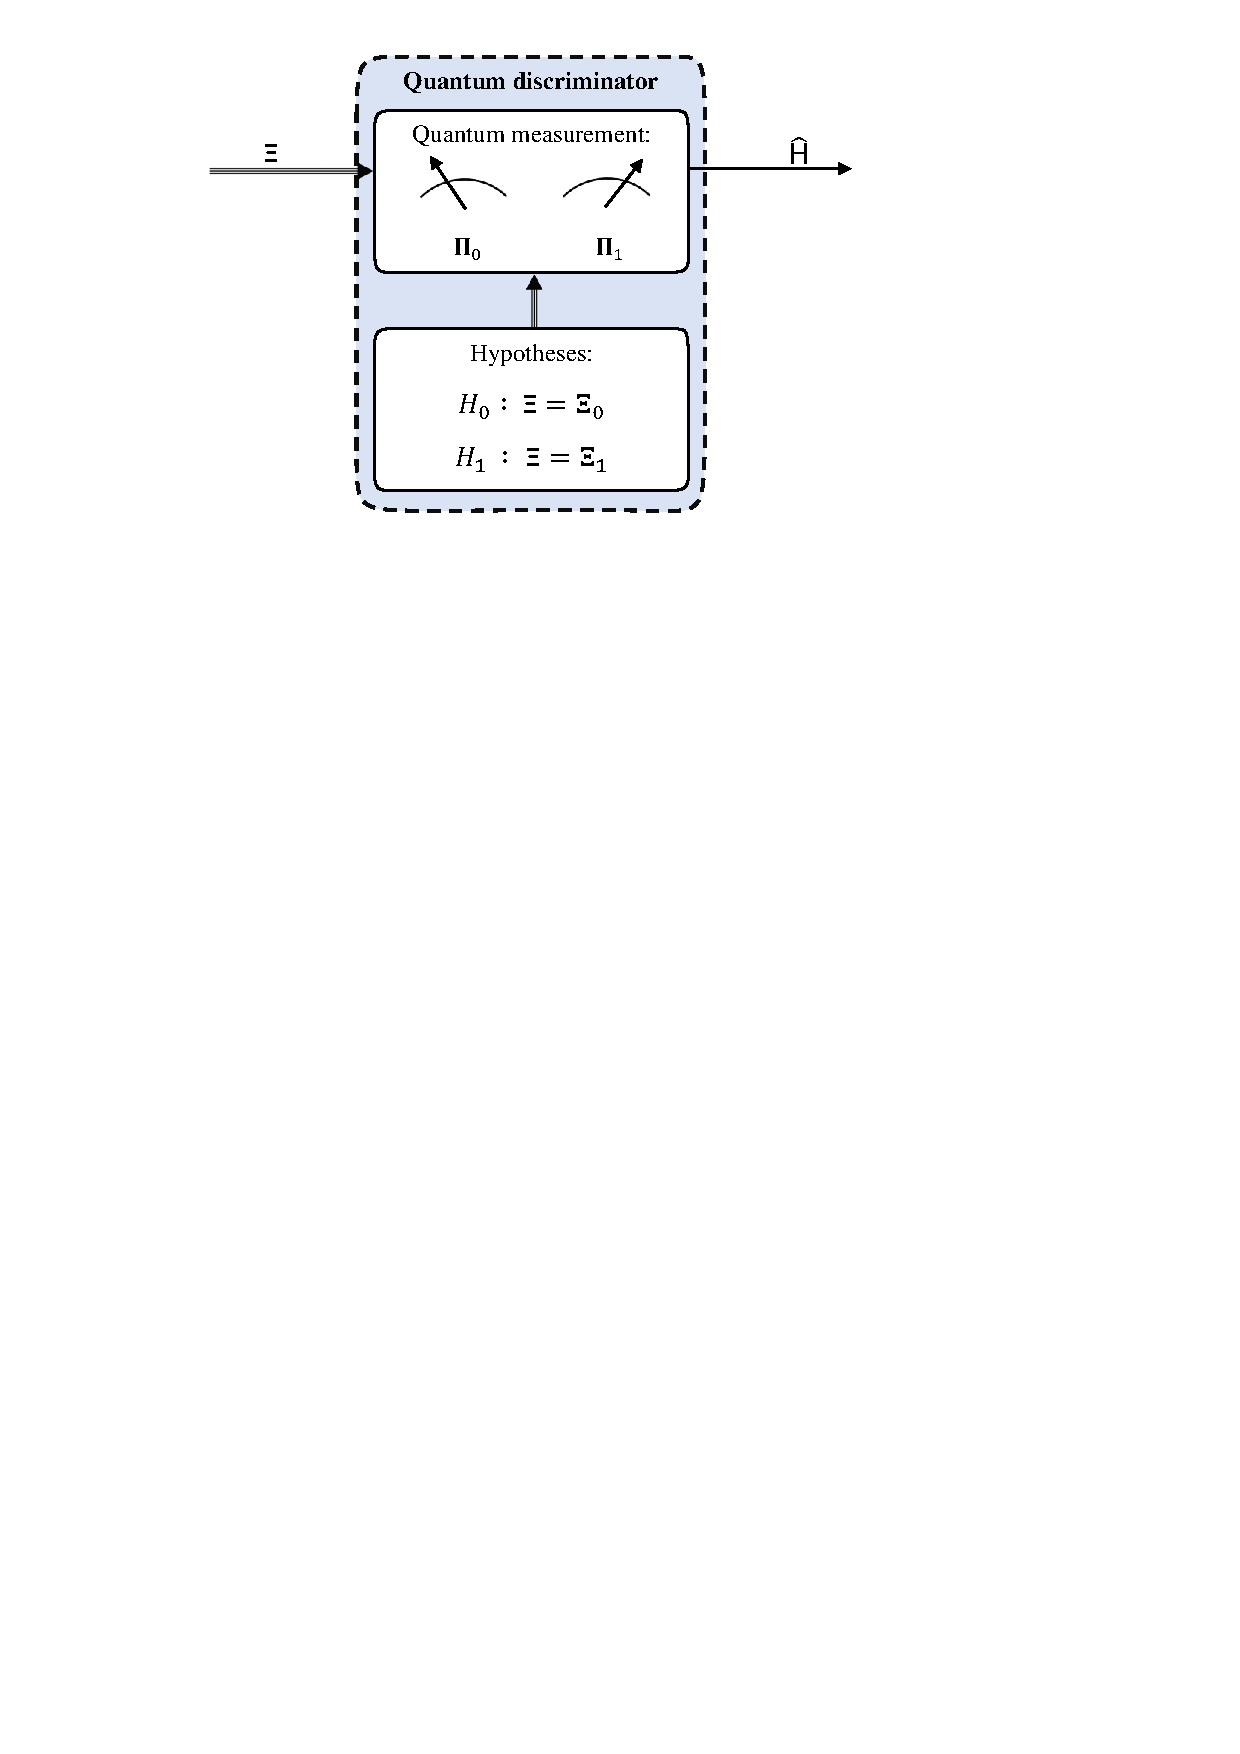
\includegraphics[width=1\textwidth]{fig2.1.pdf}
        \caption{Block diagram of a quantum transmitter.}
        \label{fig:2.1}
    \end{figure}
    It is possible to think about the quantum transmitter as in figure \ref{fig:2.1}. The bit source
    emits a bit sequence $a[n]$, the serial-parallel converter parallelizes a group of $l$-bit (where
    if $L$ is the number of quantum states, $l=\log_2(L)$) and sends them to the quantum modulator.
    This latter associates one quantum state to every group of bit. The operation of quantum state 
    creation, in real cases, is affected by noise.

    The sequence of operations is very close to a classical transmitter: the main difference is that
    the modulator maps the bits into quantum states instead of classical modulation. Therefore, it is 
    possible to achieve the quantum equivalent of classical modulation, with several states. After 
    that, the impact on performance can be tested.
    This thesis only considers and assesses the binary cases, in the OOK and BPSK 
    configuration.
    
    \subsection{OOK modulation}
        The OOK (on-off keying) is the most simple possible configuration for a communication system.
        The quantum implementation of that is realized associating the low-energy state to the 
        ground state $\ket{0}$ and the high-energy state to another state. It is important to
        consider that the physical realization of these states are not free-noise; this issue will be
        considered using noisy states \ref{eq:2.1.1}.
        \begin{equation}
            \pmb{\Xi}_0 = \pmb{\Xi}_{th}
            \label{eq:2.1.1}
        \end{equation}
        \begin{equation*}
            \pmb{\Xi}_1 = \pmb{\Xi}_{th}(\mu)
        \end{equation*}
        In the equation \ref{eq:2.1.1}, the high-energy state is associated to a coherent state. This 
        configuration has been widely analyzed in \cite{helstrom1,helstrom2,coherentComm1,coherentComm2,
        coherentComm3,coherentComm4} but this is not the only possible way. The use of PACS states 
        $\pmb{\Xi}_{th}^{(k)}(\mu)$ is analyzed in \cite{PACSDisc,tesiGuerrini}; the use of PASS are briefly
        assessed in the following chapter of this thesis.

    \subsection{BPSK modulation}
        BPSK quantum systems are implemented using two states with opposite amplitude, like
        \begin{equation}
            \pmb{\Xi}_0 = \pmb{\Xi}_{th}(-\mu)
            \label{eq:2.1.2}
        \end{equation}
        \begin{equation*}
            \pmb{\Xi}_1 = \pmb{\Xi}_{th}(\mu).
        \end{equation*}
        There is no guarantee that the use of a BPSK solution in  a quantum system will 
        improve its performance. The effect depends on which are the used states. In the next chapter some 
        configuration are assessed.

    \section{Quantum Discriminator}
    The problem of quantum state discrimination (QSD) is one of the most important
    aspects of quantum communication. As in classical communication, the ability to 
    distinguish between two or more states in presence of noise can be decisive in order to determine
    the performance of the communication system. However, differently from the classical situation,
    the discrimination can be done using a custom-designed quantum discriminator, overcoming
    the classical physics limits.

    \subsection{Binary quantum state discrimination}
    \begin{figure}[ht]
        \begin{center}
            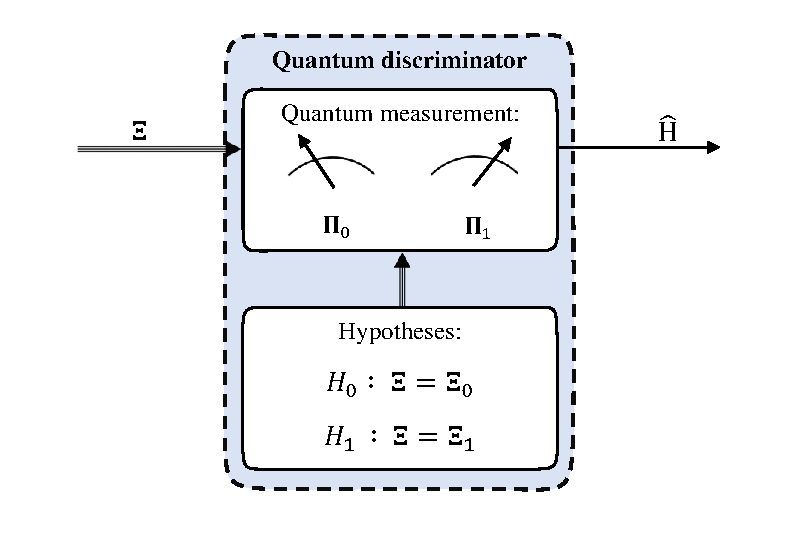
\includegraphics[width=0.75\textwidth]{fig2.2.pdf}
            \caption{Binary quantum state discriminator.}
            \label{fig:2.2}
        \end{center}
    \end{figure}
    The problem of discrimination between two quantum states is realized, as every measurement
    process \ref{post:2}, using an operator or a set of operators.
    If the state of the system is unknown, as shown in figure \ref{fig:2.2}, there are two hypotheses
    about the state $\pmb{\Xi}$ (the problem is easly generalizable for $M$ different states),
    given by:
    \begin{equation}\begin{split}
        H_0 : \pmb{\Xi}=\pmb{\Xi}_0\\
        H_1 : \pmb{\Xi}=\pmb{\Xi}_1
        \label{eq:binHyp}
    \end{split}\end{equation}
    It is necessary a set of two positive-definites operator (POVM)
    \begin{equation}
        \mathcal{P}=\{\pmb{\Pi}_0,\pmb{\Pi}_1\}
    \end{equation}
    for the discrimination process, and the probability that the hypothesis $H_j$ is choosen
    if $H_k$ is the right choose is given by \cite{tesiGuerrini}:
    \begin{equation}
        \mathbb{P}\{H_j|H_k\}=tr\{\pmb{\Xi}_k\pmb{\Pi}_j\}.
    \end{equation}
    The distribution error probability (DEP) in the discrimination process, if $p_0$ and $p_1$ are 
    respectively the probabilty of symbols $0$ and $1$, is so given by
    \begin{equation}
        P_e=1-\left(p_0 tr\{\pmb{\Xi}_0\pmb{\Pi}_0\}+p_1 tr\{\pmb{\Xi}_1\pmb{\Pi}_1\}\right).
    \end{equation}

    \subsection{Optimal discriminator}
    The issue of finding the optimal POVM that minimizes the DEP was exhaustively discuss  by Helstrom in 
    \cite{helstrom3,helstrom4}. The minimum distribution error probability (MDEP) for a binary 
    communication system is given by the well-known Helstrom bound
    \begin{equation}
        \breve{P}_e = \frac{1}{2} \left(1-\norm{p_1 \pmb{\Xi}_1 - p_0 \pmb{\Xi}_0}_1 \right),
        \label{eq:HelstromBound}
    \end{equation}
    where $p_0,\ p_1$ are the probability that the states $\pmb{\Xi}_0,\ \pmb{\Xi}_1$ are trasmitted
    and the operator $\norm{\cdot}_1$ represents the trace norm. 
    The MDEP \ref{eq:HelstromBound} is obtained with the following POVM:
    \begin{equation}
        \breve{\pmb{\Pi}}_0 = \sum_{\substack{i \\ \lambda_i<0}} \ket{\lambda_i}\bra{\lambda_i},
    \end{equation}
    \begin{equation*}
        \breve{\pmb{\Pi}}_1 = 1-\breve{\pmb{\Pi}}_0 = 
        \sum_{\substack{i \\ \lambda_i \geq 0}} \ket{\lambda_i}\bra{\lambda_i};
    \end{equation*}
    where $\ket{\lambda_i}$ is the eigenvector of $p_1 \pmb{\Xi}_1 - p_0 \pmb{\Xi}_0$ associated to 
    the eigenvalue $\lambda_i$.
    For pure states, i.e $\pmb{\Xi}_0 = \ket{\psi_0}\bra{\psi_0}$ and $\pmb{\Xi}_1 = \ket{\psi_1}
    \bra{\psi_1}$, the equation \ref{eq:HelstromBound} begin
    \begin{equation}
        \breve{P}_e = \frac{1}{2} \left(1- \sqrt{1-4 p_0 p_1 \absolutevalue{\braket{\psi_0}{\psi_1}}^2}
        \right).
        \label{eq:HelstromBPure}
    \end{equation}
    It is possible to observe that, for pure states, the MDEP is equal to $0$ if $\braket{\psi_0}{\psi_1}$,
    that is $\ket{\psi_0}$ and $\ket{\psi_1}$ are orthogonal states.
    % Risultati ottenuti

\chapter{Communication with Photon Added States}
    % Conclusioni

\chapter{Conclusion}
    Questa tesi si pone come obiettivo di analizzare le prestazioni nella QSD (Quantum states discrimination) per 
    sistemi binari, in termini di probabilità di errore nel riconoscimento dei simboli, con l'utilizzo di un discriminatore ottimo.
    Sono stati presentati inizialmente i fondamenti della teoria meccanica quantistica nella formulazione di 
    Dirac-Neumann e nella sua generalizzazione tramite l'utilizzo di Density operator. Sono stati quindi descritti
    i concetti di modulazione quantum e di discriminazione di stati quantistici ed infine sono state analizzate le
    prestazioni di alcuni sistemi in termini di minimum distribution error probability (MDEP). 
    Tutte le valutazioni sono state fatte supponendo che la comunicazione non risenta di effetti associati al canale di comunicazione,
    dunque che lo stato emesso dal trasmettitore giunga al discriminatore del ricevitore senza modifiche.

    Questa tesi pone in evidenza come l'utilizzo di stati non Gaussiani (non-Gaussian states) photon added in sistemi OOK può 
    apportare un miglioramento nella QSD rispetto all'utilizzo di stati Gaussiani. La combinazione in particolare di squeezing 
    e photon addition (PASSs) risulta estremamante efficace.
    L'effetto della photon addition si manifesta invece negativo in sistemi quantistici BPSK.

    I risultati ottenuti possono essere di notevole importanza nel design di un sistema di comunicazione che sfrutti stati 
    quantistici, permettendo di sfruttare al meglio le potenzialità di questa teoria fisica.

    \bibliographystyle{IEEEtran}
    \bibliography{bibliography}
    
    %\printbibliography[heading=bibintoc]
\end{document}